\documentclass[../sparc.tex]{subfiles}
\graphicspath{{\subfix{../images/}}}
\begin{document}

\section{Potential Difference}
\index{Electronics!Potential Difference}

Let's take another look on fig. \ref{fig:electronics-circuits-1}.  Water flowing
from vessel ``A'' to vessel ``B'' through a pipe.  As soon as the water levels
equalize the water flow will stop (see fig. \ref{fig:electronics-circuits-2}.)

\begin{figure}[ht]
  \centering
  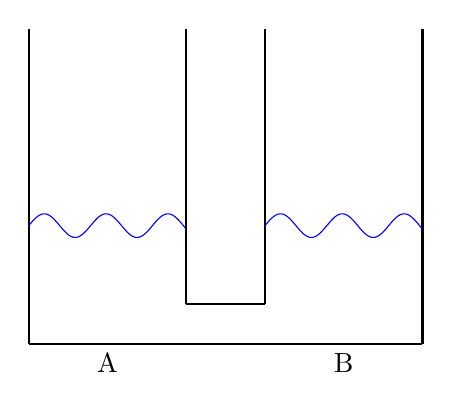
\begin{tikzpicture}[
      declare function={f1(\x) = 0.15 * sin(8.0 * deg(\x));
    }]

    \draw[thick] (0, 0) -- (0, 4);
    \draw[thick] (2, 0.5) -- (2, 4);
    \draw[thick] (0, 0) -- (2, 0);

    \draw[thick] (3, 0.5) -- (3, 4);
    \draw[thick] (5, 0) -- (5, 4);
    \draw[thick] (3, 0) -- (5, 0);

    \draw[thick] (2, 0) -- (3, 0);
    \draw[thick] (2, 0.5) -- (3, 0.5);


    \begin{scope}[yshift=1.5cm, color=blue]
      \draw (0, 0) plot[domain=0:2, variable=\x, samples=200, smooth] ({\x}, {f1(\x)});
    \end{scope}

    \begin{scope}[yshift=1.5cm, xshift=3cm, color=blue]
      \draw (0, 0) plot[domain=0:2, variable=\x, samples=200, smooth] ({\x}, {f1(\x)});
    \end{scope}

    \draw (1, 0) node[below] {A};
    \draw (4, 0) node[below] {B};

  \end{tikzpicture}
  \caption{An example of two vessels with the equal level of water.}
  \label{fig:electronics-circuits-2}
\end{figure}

A similar situation to this is when a battery is discharging.  There are
chemical reactions going inside the battery when it is in usage; the chemical
reactions produce the voltage level difference between positive and negative
battery contacts.  In electronics we say that there is a \emph{potential
difference}.  Those chemical reactions getting slower and less potent with time,
up to the moment when battery cannot give enough current to power up an electric
circuit.

Thus, we can conclude that the third condition for electric current flow is the
presence of a potential difference in the circuit.

An interesting fact: for electric current to flow it is not necessary to have a
voltage difference between some positive value and zero.  See, it is important
to have voltage difference in the first place, but the levels can vary.  For
example, we can make a circuit with voltage difference of 5 Volts in many ways:
it could be a difference between 5V and 0V, 10V and 5V or even 2.5V and -2.5V.
It turns out that the voltage can be negative and it is quite normal thing to
see in electronics.

If we draw our analogy with water further, we can imagine that we can make water
flow between two vessels with the same amount of water by placing one of them
higher than the other, thus making a ``potential difference''.  This water flow
will continue until the water levels will be in equilibrium again (see
fig. \ref{fig:electronics-circuits-3}.)

\begin{figure}[ht]
  \centering
  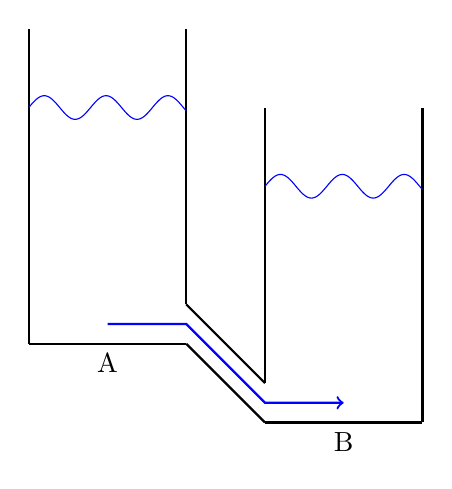
\begin{tikzpicture}[
      declare function={f1(\x) = 0.15 * sin(8.0 * deg(\x));
    }]

    %% 1st vessel.
    \draw[thick] (0, 0) -- (0, 4);
    \draw[thick] (2, 0.5) -- (2, 4);
    \draw[thick] (0, 0) -- (2, 0);

    %% 2nd vessel.
    \draw[thick] (3, -0.5) -- (3, 3);
    \draw[thick] (5, -1) -- (5, 3);
    \draw[thick] (3, -1) -- (5, -1);

    %% Pipe
    \draw[thick] (2, 0) -- (3, -1);
    \draw[thick] (2, 0.5) -- (3, -0.5);

    \draw[thick, color=blue, ->]
    (1, 0.25) -- (2, 0.25) -- (2, 0.25) -- (3, -0.75) -- (4, -0.75);


    \begin{scope}[yshift=3cm, color=blue]
      \draw (0, 0) plot[domain=0:2, variable=\x, samples=200, smooth] ({\x}, {f1(\x)});
    \end{scope}

    \begin{scope}[yshift=2.0cm, xshift=3cm, color=blue]
      \draw (0, 0) plot[domain=0:2, variable=\x, samples=200, smooth] ({\x}, {f1(\x)});
    \end{scope}

    \draw (1, 0) node[below] {A};
    \draw (4, -1) node[below] {B};

  \end{tikzpicture}
  \caption{An example of vessels with the equal amount of water but different
    levels.}
  \label{fig:electronics-circuits-3}
\end{figure}

In electronics it is sufficient to have any potential difference for current to
flow.  Some examples of potential is shown in table
\ref{table:electronics-potential-difference}.  As you can see from the table you
can power up a regular LED using 1003.3V and 1000V as the potential difference
will be just 3.3V (the same as an Arduino can provide.)

\begin{table}[h]
  \centering
  \begin{tabular}{c | c | c}
    Upper voltage & Lower voltage & Potential Difference \\
    \hline
    5V & 0V & 5V \\
    \hline
    10V & 5V & 5V \\
    \hline
    5V & -5V & 10V \\
    \hline
    1003.3V & 1000V & 3.3V \\
    \hline
  \end{tabular}
  \caption{Some examples of possible potential difference.}
  \label{table:electronics-potential-difference}
\end{table}

\end{document}
